\documentclass{article}
\usepackage[a4paper, total={5.5in, 9in}]{geometry}
\usepackage{times}
\usepackage{pgfplots}
\usepackage{harpoon}
\usepackage{tikz}
\pgfplotsset{compat=1.18}

%-------Create Gauss function for plotting------------------------%
\newcommand\gauss[2]{1/(#2*sqrt(2*pi))*exp(-((x-#1)^2)/(2*#2^2))}
%-----------------------------------------------------------------%


\begin{document}
    \title{Modelling changes of phenotypic distribution in natural populations due to selection by means of computer algorithm}
    \author{Kári Hlynsson}
    \date{\today}
    \maketitle

    \begin{abstract}
        \noindent In this paper we discuss the uses of computer simulation in predicting the change of phenotypic distributions in natural populations as a result of natural selection. By means of statistical analysis and data visualization, we propose a method with which certain evolutionary patterns in populations can be identified. All the findings of this publication are not meant to reflect the exact mechanisms of natural selection and precisely how adaption occurs but aims to display generally how traits in populations develop over time and react to new environmental factors. 
    \end{abstract}

    \section*{Introduction}
    \subsection*{Algorithm construction}
    The algorithm used to simulate conditions presented in this paper was programmed using Python 3.9.5. Live plotting was accomplished by utilization of Matplotlib. However, in case of data visualization post-simulation, R was used. The author of this paper would like to note that the intent of this simulatory algorithm is not to reflect precisely how adaptation in species occurs but rather to display generally how the mechanisms of natural selection operate. 
    \par We begin by considering a population $P$ of $n$ individuals. All individuals of $P$ share similir traits such as lifespan and number of offspring produced. Table 1 below shows some of the definitions of various traits that will be used in this algorithm. 
    \begin{table}[h]
        \small
        \centering
        \renewcommand{\arraystretch}{1.2}
        \begin{tabular}{| c | l | p{.5\textwidth} |}
            \hline
            \textbf{Symbol} & \textbf{Trait} & \textbf{Description} \\
            \hline
            $P$ & Population & Set of individuals of the same species. \\
            $E$ & Environmental difficulty & Factor present in environment which affects survival or fertility of individual in population. \\
            $\varsigma$ & Selection ratio & Ratio of individuals selected for environmental checks and total population size. \\
            \hline
            $i$ & Individual & Individual organism of population $P$. \\
            $w_i$ & Fitness & An individual's fitness towards the environment. \\
            $w_{\overline{z}}$ & Comparative fitness & The ratio of an individual's fitness and the modal fitness value $\overline{z}$ of population $P$. \\
            $\lambda$ & Reproductive capability & Number of offspring produced per individual. \\
            $\tau$ & Genetic volatility & The likelihood that the offspring of an individual $i$ will express drastic changes in phenotype and thus greatly affect fitness.
        \end{tabular}
        \caption{Abbreviatons and symbols used for algorithm variables.}
    \end{table} 
    \par \noindent The algorithm is \emph{turn-based} in the sense that individuals perform certain tasks and are exposed to environmental factors on a single-turn basis. By using this method, we can clearly visualize and analyze data gathered from simulations to estimate various factors in adaptation of the population to the specific environment. Thus when we say that the time elapsed is 500 intervals, we are referring speficically to how many \emph{time intervals} or \emph{turns} have passed from the start of the simulation. For the sake of simplicity, henceforth we shall refer to these intervals as \emph{time intervals}.
    \par An algorithmic component that requires careful consideration is how to determine \emph{whether an individual survives in the environment or not}. While there are many ways to do this, we shall utilize an \emph{environmental factor}, $E$, to carry out the logical comparison
    \begin{equation}
        P(w_i) = w_i \geq E
    \end{equation}
    \par \noindent If $P(w_i)$ for a given individual is true, that individual is said to have \emph{survived the environmental check}. Else, it is said to have failed and will be removed from the population, effectively \emph{dying}. By specifying a selection ratio, $\varsigma$, upon initial configuration, the percentage of the population that is selected each turn can be modified.
    \par At the onset of each turn, all individuals who have attained the max age of their species will die. All individuals who survive the environmental check in the following turn are prompted to reprduce. If their \emph{reproductive cooldown} timer has not reached zero, they will not reproduce that turn. Those that do reproduce produce $\lambda$ offspring. Calculation of offspring fitness is acquired by the formula
    \begin{equation}
        w_c = w_p \pm \rho
    \end{equation}
    Where $\rho$ is uniformly a trivial shift in fitness to represent shuffling of genetic material and such. However, acquired \emph{genetic volatility} depicted by the variable $\tau$ presents the probability of a \emph{mutation} occuring when an individual reproduces. A mutation has a more drastic effect on an individual's fitness and can be either deleterious or beneficial.
    \subsection*{Data analysis}
    We shall start this section by defining some key parameters that shall be used in the calculations of this paper. One variable of interest is the \emph{modal location of the fitness value} in a population, which we symbolize $\overline{z}$. By studying the displacement of this location, we can see how much adaptation has taken place as a result of exposure to an environmental factor.
    \begin{figure}[h]
        \centering
        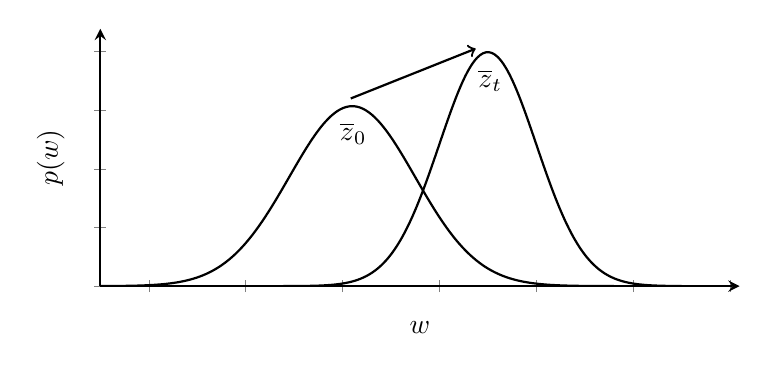
\begin{tikzpicture}[]
       		\begin{axis}[
                xlabel={$w$},
                ylabel={$p(w)$},
				width=0.8\textwidth,
				height=0.4\textwidth,
                xticklabels=\empty,
                yticklabels=\empty,
				domain=-5:7,
				axis x line=bottom,
				axis y line=left,
				samples=200,
                thick,
				smooth,
				enlargelimits=upper
			]
                \addplot[mark=none, thick]{\gauss{0.2}{1.3}};
				\addplot[mark=none, thick]{\gauss{3}{1.0}};
                \draw[thick, ->] (0.17, 0.32) to (2.75, 0.405);
                \node (z0) at (0.22, 0.26) {$\overline{z}_0$};
                \node (zt) at (3.05, 0.35) {$\overline{z}_t$};
			\end{axis} 
        \end{tikzpicture}
        \caption{Determination of $\Delta \overline{z}$ can be used as indicator of adaptation.}
    \end{figure}
    \par \noindent Figure 1 depicts the vector displacement of $\overline{z}$ at simulation start ($t = 0$) towards $\overline{z}_t$, that is when $t$ time intervals have passed. We can represent the displacement with the vector notation
    \begin{equation}
        \overrightharp{F}_S = \pmatrix{\Delta \overline{z}_x \cr \Delta \overline{z}_y} = \pmatrix{\overline{z}_{x(t)} - \overline{z}_{x(0)} \cr \overline{z}_{y(t)} - \overline{z}_{y(0)}}
    \end{equation} 
    \par \noindent and define it as the \emph{force of selection} due to environmental factor $E$. This provides us with a variable that allows for quantitative observation of the mechanisms of selection within the algorithm. Note that a high x value of a $\overrightharp{F}_S$ indicates that the \emph{adaptive magnitude} was very high while a high y value indicates that the \emph{adaptive saturation} is very dense.
    \par An interesting facet of the algorithm that presented itself despite its unintended appearance in the simulation is the \emph{relationship between birth/death rate and carrying capacity}. Imagine that $n_d$ individuals die each turn while $n_b$ are born into the population. Due to the algorithm's construction we can reasonably estimate the number of individuals born into the population each turn by usage of the reproductive capability constant $\lambda$ and the number of \emph{individuals who are capable of producing each round}.
    \begin{equation}
        n_b = \lambda n_r
    \end{equation}
\end{document}

